
\section{Profile Hidden Markov Model}

This section focuses on the main parts of \ac{pHMM}, including \ac{MSA} and scoring methods. More background, especially regarding the fundamentals of \acp{HMM} such as Markov chains, can be found in \cite{Durbin.1998, Baldi.2001}.  

\subsection{Multiple Sequence Alignment (MSA)}
\label{sec:MSA}

The \ac{pHMM} used for homology detection is initialized by a set of protein sequences that are aligned to each other for a high degree of structural similarity.

Two sequences can be compared by a pairwise sequence alignment, where the residues of both sequences are directly compared to each other, allowing for the use of gap positions between the residues. Two protein sequences are highly similar when they have many match-states of the same or similar amino acid residues and few gaps. Sequences with high similarity are also highly likely to be homologous and display structural and evolutionary conservation. 
An \ac{MSA} arranges three or more sequences to one another. This method is especially commonly used on a set of sequences that are related to one another in order to identify homologous residues or sequence patterns that may have diverged from common ancestral residues.  
Functionally important residues in a sequence are assumed to remain stable over generations and are less likely to mutate. Therefore, highly conserved regions, with high similarities over the columns of the \ac{MSA}, are identified as functionally important. With a higher number of homologous sequences in an \ac{MSA}, common residues can be identified with a higher probability, while  the likelihood of random similarities occurring decreases.
Nevertheless, a low sequence similarity does not imply that these sequences are not homologous. Positions of the \ac{MSA} can be conserved by additional parameters, such as \ac{PP}. For example, a column or region of the \ac{MSA} that only contains hydrophobic residues is likely to serve a water-repelling function in the protein. 
For certain proteins, the homology based on its sequence is not obvious, but a similar three-dimensional structure and function may imply a common evolutionary origin. 
  Figure \ref{fig:MSA} shows an \ac{MSA} composed of 15 sequences from the same superfamily (see Section \ref{sec:SCOP}).

\begin{figure}[h!]
	\begin{center}
		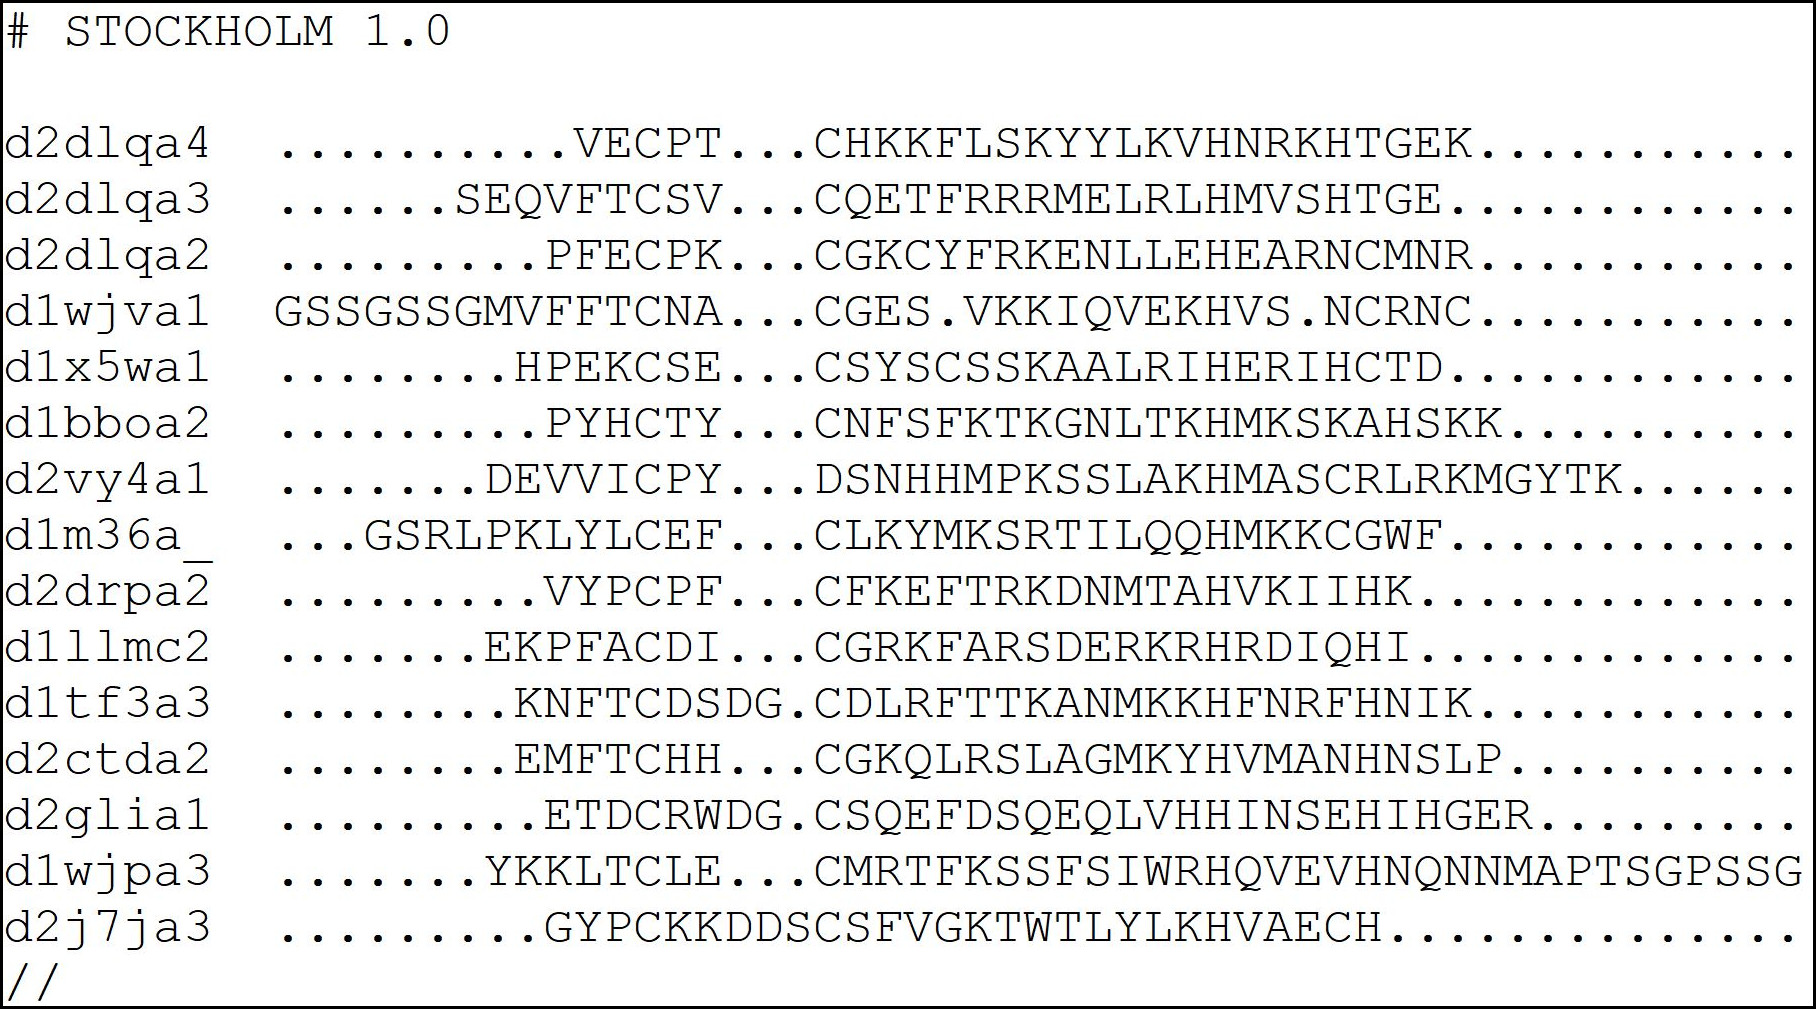
\includegraphics[width=0.8\textwidth]{fig/MSA}
	\end{center}
	\caption{Fifteen sequences from the \acs{SCOP} superfamily g.37.1 aligned to an \acs{MSA}.}
	\label{fig:MSA}
\end{figure}



There are different approaches for generating an \ac{MSA}, using either manual annotation by expert knowledge or automatic methods based on structural information on its different levels (see \cite[Chapter~6]{Durbin.1998}).


\subsection{Profile Hidden Markov Model}

A \ac{pHMM} is a stochastic  model based on Markov chains used especially in bioinformatics to model an \ac{MSA} and capture its degree of structural conservation.   Figure \ref{fig:pHMM} shows the structure of a \ac{pHMM}, which uses three different types of hidden states for each column of the \ac{MSA}. These are match state $M_k$, delete state $D_k$ and insert \mbox{state $I_k$.}

\begin{figure}[h!]
	\begin{center}
		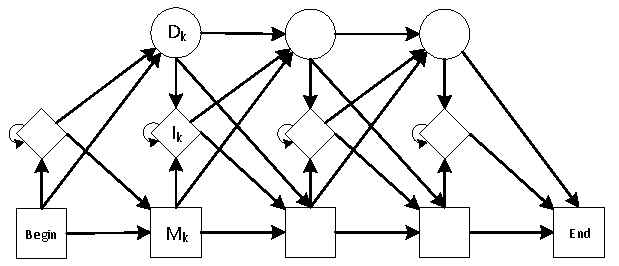
\includegraphics[width=0.85\textwidth]{fig/pHMM}
	\end{center}
	\caption[Structure of a pHMM.]{Structure of a \acs{pHMM} with match, insert and delete states, adapted from \cite{Durbin.1998}.}
	\label{fig:pHMM}
\end{figure}


Match state $M_k$ is described by a distribution, trained with the symbol frequency in column $k$ of the \ac{MSA}. Each representative column in the \ac{MSA} model matches one state. Gaps in the MSA influence the insertion and deletion states.

Insertion states model genetic insertions of additional symbols in a sequence that do not appear in the majority of the sequences of a family of proteins in the \ac{MSA}.
They occur when there are many gaps in a column, typically above 50\,\%. Insertion states  make it possible to insert the symbols in the \ac{MSA} for those sequences that do not show gaps.
Insertion states have a self-transition to cover repeated insertions over multiple columns. 
Instead of the actual symbol frequency of the \ac{MSA} column, the emission probabilities can be set to a background probability based on a general frequency of the symbols, as a few residues in the column might not be representative.

Deletions allow a sequence to skip over a match state without emitting a symbol and model situations of genetic deletions, where a certain sequence has one or more positions fewer than the other proteins in a family modeled by the \ac{MSA}.
Deletions are silent states without emitting symbol probabilities. Self-transitions are not allowed  for deletions. However, gaps over multiple columns are modeled as a sequence of deletion states, allowing different transition probabilities over multiple gap positions.


\subsection{Decoding and Scoring}
\label{sec:scoringTh}

In a fully defined \ac{pHMM}, any sequence can be represented by a matching score, by multiplying the transition and emission probabilities along the path. Due to the insert and delete states, many different paths can produce the same sequence. To find the \mbox{best-suited} path for a specific sequence, dynamic programming approaches are used, such as the \textit{forward algorithm} or the \textit{Viterbi algorithm}.

The forward algorithm calculates the overall probability as a sum for each individual state of the \ac{pHMM}. 
The Viterbi algorithm calculates the probability for the most likely sequence of states by using the maximized path over the \ac{pHMM}.

To prevent an underflow caused by the multiplication of many probabilities in the range of 0--1, a logarithmic scale is used to calculate the raw score. However, these raw scores are highly dependent on the overall sequence length, as longer sequences generate smaller scores, and thus these raw scores are difficult to compare. Therefore, the scores can be normalized using correction methods such as null models, which can either be simple null models or reversed-sequence null models. The simple null model uses a simplified one-state \ac{HMM} with a specific residue composition based on general occurrence frequencies of the amino acids and scores the sequence against it. The reversed-sequence null model uses the original \ac{pHMM} and scoring algorithm, but reverses the direction of the sequence employed. The final score without length dependency is calculated by subtracting the null model score from the raw score in the logarithmic scale.